\chapter{静电学中的边界条件问题}
\label{chap:boundary-value problems}

静电学中最为常见的问题,便是给定边界条件,求解某区域中的电场、电势、电荷密度等。
在\secref{ssec:Green solve Poisson}中,我们已经介绍了Green函数法求解Poisson方程,并给出了不同边界条件下的形式解。但是%我们知道,
从形式解很难得到具体问题的通解,因为Green函数的具体形式未知,其与边界形状、边界条件有关。%相似问题的Green函数往往大相径庭。
因此,便发展起许多求解静电学边值问题的方法,这些内容其实也是数学物理方法中的重要部分。

% Jackson将这些方法分为两个章节讲述。本人认为这种分类意义不大,故此笔记将其作为一个章节记录。

\paragraph{第一部分}

本部分主要介绍其中的三个方法:\secref{sec:method of images}的电像法、\secref{sec:orthogonal functions and expansions}的正交函数展开法(分离变量法)、\secref{sec:finite element analysis}的有限元分析法。
限于篇幅,Jackson省略了复变函数方法。%后续如果有时间,
% 保角变换法和积分变换法可参见本人复变函数笔记。

\usetikzlibrary{circuits.ee.IEC}

\section{电像法}
\label{sec:method of images}

%通过添加镜像电荷,使边界上的电位满足特定条件。
电像法(method of images)用于求解一个或多个点电荷在特定边界$\p V$内的问题。在边界$\p V$形状较好的条件下,可以在$V$外\footnote{镜像电荷必须在$V$外部,否则它们的存在将改变$V$内实际电荷的排列,违反Poisson方程。}添加适当的点电荷来模拟所需的边界条件,这种虚拟电荷称为镜像电荷(image charge)。
\begin{example}{接地无限平面导体的镜像电荷}{method of images, infinite plane conductor}
    一个简单的例子是接地无限平面导体前的点电荷$q$,如下图所示。移除原边界并对称地放置一镜像电荷$q'=-q$后,即可满足原平面所在位置电势为0。
    \begin{center}
        \begin{tikzpicture}[circuit ee IEC]
            \fill[pattern=north east lines](-.3, 0)rectangle(0, 4);
            \draw[thick](0, 0)--(0, 4)node[right]{$\Phi=0$};
            \draw (0, 0.5) to (0.8, 0.5) to [ground={at end}] (0.8, 0.15);
            \draw[dashed](0, 2)--(2, 2)node[below]{$d$};
            \fill[black](2, 2)circle(.05)node[above]{$q$};
        \end{tikzpicture}\qquad
        \begin{tikzpicture}
            \draw[dashed](0, 0)--(0, 4)node[right]{$\Phi=0$};
            \draw[dashed](-2, 2)--(2, 2);
            \fill[black](2, 2)circle(.05)node[above]{$q$};
            \fill[black](-2, 2)circle(.05)node[above]{$q'$};
        \end{tikzpicture}
        \captionof{figure}{电像法}
        \label{fig:image charge of plane}
    \end{center}
    因此电势分布为
    \begin{equation}
        \Phi(\bm x)=\frac q{4\pi\varepsilon_0}\biggkh{\frac1{\abs{\bm x-\bm d}}-\frac1{\abs{\bm x+\bm d}}}.
    \end{equation}
\end{example}

\subsection{球导体的电像法}
\label{ssec:method of images, sphere}

对于球导体也可采用电像法,其背后的几何意义为Apollonius圆的定义:平面内到两定点距离的比值为定值的点轨迹构成一个圆。%\footnote{\url{https://en.wikipedia.org/wiki/Circles_of_Apollonius}}

\begin{example}{接地导体球的镜像电荷}{method of images, grounded sphere conductor}
    一半径为$a$的导体球接地,球外有一电荷$q$,距球心$d>a$
    \begin{center}
        \begin{tikzpicture}[circuit ee IEC]
            \fill[even odd rule, pattern=north east lines](0, 0)circle(1.5)(0, 0)circle(1.3);
            \draw[thick](0, 0)circle(1.5);
            \draw (1.2, -.9) to (2, -.9) to [ground={at end}] (2, -1.5);
            \draw[dashed](0, 0)node[left]{$O$}--(4, 0);
            \fill[black](4, 0)circle(.05)node[below]{$d$}node[above]{$q$};
        \end{tikzpicture}
        \captionof{figure}{接地导体球和点电荷}
        \label{fig:sphere conductor}
    \end{center}
    我们可以在球壳内放置一镜像电荷$q'$,由对称性,$q'$一定在$q$与球心的连线上:
    \begin{center}
        \begin{tikzpicture}
            \draw[dashed](0, 0)circle(1.5);
            \draw[dashed](0, 0)node[left]{$O$}--(4, 0);
            \fill[black](4, 0)circle(.05)node[below]{$d$}node[above]{$q$};
            \fill[black](.5625, 0)circle(.05)node[below]{$d'$}node[above]{$q'$};
        \end{tikzpicture}
        \captionof{figure}{镜像电荷}
        \label{fig:image charge of sphere}
    \end{center}
    不难验证,取
    \begin{equation}
        \label{eqn:image charge of sphere}
        q'=-\frac adq,\quad d'=\frac ada.
    \end{equation}
    便可使原球面上的电势均为0,因此球外电势分布为
    \begin{equation}
        \Phi(\bm x)=\frac q{4\pi\varepsilon_0}\biggkh{\frac1{|\bm x-\bm d|}-\frac ad\frac1{|\bm x-\bm d'|}},\quad\bm d'=\Bigkh{\frac ad}^2\bm d.
    \end{equation}
    \tcblower
    接地导体球外表面的面电荷密度为($\p V$上的法向量$n'$指向球内,即$-r$方向)
    \begin{equation}
        \label{eqn:grounded sphere conductor-point, sigma}
        \sigma=-\varepsilon_0\edg{\pv\Phi r}_{r=a}=-\frac q{4\pi a}\frac{d^2-a^2}{(d^2+a^2-2ad\cos\theta)^{3/2}}.
    \end{equation}
    球体上的总感应电荷等于像电荷$q'$,这可以根据Gauss定律直接得出,也可以对$\sigma$在$\p V$上积分得到。

    作用在电荷$q$上的力等于电荷$q$和像电荷$q'$之间的Coulomb力:
    \begin{equation}
        \label{eqn:grounded sphere conductor-point, F}
        F=\frac1{4\pi\varepsilon_0}\frac{qq'}{(d-d')^2}=\frac{q^2}{4\pi\varepsilon_0}\frac{ad}{(d^2-a^2)^2}.
    \end{equation}
    也可以将$\sigma^2/2\varepsilon_0$在$\p V$上积分得到。
\end{example}

\begin{remark}
    这个结果同样适用于球内的电荷($y<a$)。唯一需要改变的是\eqref{eqn:grounded sphere conductor-point, sigma},其中导体外的法向导数现在是径向向内的,这意味着符号的变化。导体球内表面感应电荷为$-q$,与$d$无关。
\end{remark}

\begin{example}{带电孤立导体球的镜像电荷}{method of images, charged sphere conductor}
    将\exmref{exm:method of images, grounded sphere conductor} 的导体球换为总电荷为$Q$的孤立导体球,可以用线性叠加法建立电势的解:
    \begin{compactenum}
        \item 首先将导体球接地,即\exmref{exm:method of images, grounded sphere conductor} 得到的结果;
        \item 然后切断导体球的接地,导体球外表面会带上$q'$的电荷,我们只需要再向外表面添加$(Q-q')$的电荷即可,由于导体是等电位的,这些$(Q-q')$电荷将均匀地分布在外表面上。
    \end{compactenum}
    因此电势会添加一项等效于处于原点的$(Q-q')$点电荷的电势。
    
    而原点电荷受到的力为
    \begin{equation}
        F=\frac1{4\pi\varepsilon_0}\frac q{d^2}\biggfkh{Q-q\frac{a^3(2d^2-a^2)}{d(d^2-a^2)^2}}.
    \end{equation}
    当$y\gg a$时,电场力会退化为两个点电荷之间的Coulomb力
    \[
        F\simeq\frac1{4\pi\varepsilon_0}\frac{qQ}{d^2}.
    \]
    当$Q\gg q$时,相互作为用0的点(不稳定平衡点)坐标$y$为
    \begin{equation}
        Q\simeq\frac{qa^2}{4(d-a)^2}\implies d\simeq a\biggkh{1+\frac12\sqrt{\frac qQ}}.
    \end{equation}
\end{example}
\begin{remark}
    当点电荷处于导体球内时,由Gauss定律,导体球内表面会产生$-q$的感应电荷。因此若导体球带总电荷为$Q$时,其外表面电荷应为$Q+q$,且均匀地分布在外表面。
\end{remark}
\begin{example}{固定电势导体球的镜像电荷}{method of images, sphere conductor at fixed potential}
    将\exmref{exm:method of images, grounded sphere conductor} 的导体球换为电势为$V$的导体球,类似于\exmref{exm:method of images, charged sphere conductor},但额外加在导体球上的电荷$(Q-q')$应改为$(4\pi\varepsilon_0\cdot Va)$。
\end{example}
\begin{example}{电像法处理匀强电场中的导体球问题}{method of images, sphere conductor in uniform E}
    考虑均匀电场$E_0$中半径为$a$的导体球。均匀场可以认为是在无穷远处由带适当电荷的正负电荷产生的,如下图所示
    \begin{center}
        \begin{tikzpicture}
            \draw[dash dot](-5, 0)--(5, 0);
            \fill[black](4, 0)circle(.05)node[above]{$-Q$}node[below]{$+R$};
            \fill[black](-4, 0)circle(.05)node[above]{$+Q$}node[below]{$-R$};
            \draw[dashed](-4, 0)--(0, .8)--(4, 0);
            %\draw[thick, <->](1, 1)--(0, .8)--(1, .6);
            \draw[thick, ->](0, .8)--(2, .8)node[above]{$\bm E_0$};
        \end{tikzpicture}
        \captionof{figure}{正负电荷近似匀强电场}
        \label{fig:uniform E approx +-q}
    \end{center}
    有两个电荷$\pm Q$,位于$\mp R$位置,在原点附近电场可以近似为均匀。
    \[
        E_0\simeq\frac1{4\pi\varepsilon_0}\frac{2Q}{R^2}.
    \]
    保持$Q/R^2$不变,在$R,Q\to\infty$的极限下,这个近似是精确的。

    因此使用电像法的结论,构造两个镜像电荷$\pm Qa/R$,得到球坐标系下的电势$\Phi(r,\theta)$,
    \iffalse
    \begin{align*}
        \Phi(r,\theta)=\frac1{4\pi\varepsilon_0}\Bigg[\frac{Q}{(r^2+R^2+2Rr\cos\theta)^{1/2}}-\frac{Q}{(r^2+R^2-2Rr\cos\theta)^{1/2}}\\
        -\frac{aQ}{R\biggkh{r^2+\dfrac{a^4}{R^2}+2\dfrac{a^2}Rr\cos\theta}^{1/2}}+\frac{aQ}{R\biggkh{r^2+\dfrac{a^4}{R^2}-2\dfrac{a^2}Rr\cos\theta}^{1/2}}\Bigg].
    \end{align*}
    \fi
    由于$R\gg r$,可进行Taylor展开:
    \begin{align}
        \notag
        \Phi(r,\theta)&=\frac1{4\pi\varepsilon_0}\frac{2Q}{R^2}\biggkh{-r\cos\theta+\frac{a^3}{r^2}\cos\theta+\mathcal O\biggkh{\frac1R}}\\
        &=-E_0\biggkh{r-\frac{a^3}{r^2}}\cos\theta.
    \end{align}
    省略的部分内容随着$R\to\infty$而消失。则导体球的面电荷密度为
    \begin{equation}
        \sigma=-\varepsilon_0\edg{\pv\Phi r}_{r=a}=3\varepsilon_0E_0\cos\theta.
    \end{equation}
    电荷密度的面积分为0,因此导体球接地与否没有区别。
\end{example}

\subsection{球边界的Green函数}
\label{ssec:Green function, sphere}

对于球形Dirichlet边界条件,为了使球面上的$G(\bm x,\bm x')=0$,可借助镜像电荷的思想,取
\begin{equation}
    \label{eqn:sphere Green function}
    G(\bm x,\bm x')=\frac1{|\bm x-\bm x'|}-\frac a{x'}\frac1{|\bm x-\bm x''|},\quad\bm x''=\Bigkh{\frac{a}{x'}}^2\bm x'.
\end{equation}
令$\gamma$表示$\bm x,\bm x'$夹角,则
\[
    G(\bm x,\bm x')=\frac1{(x^2+x'^2-2xx'\cos\gamma)^{1/2}}-\frac a{(x^2x'^2+a^4-2a^2xx'\cos\gamma)^{1/2}},
\]
式\eqref{eqn:Dirichlet Green}中还需要$\p G/\p n'$,若感兴趣的区域为球外,则$n'$指向球内,
\begin{equation}
    \label{eqn:sphere dGreen function}
    \edg{\pv G{n'}}_{x'=a}=-\edg{\pv G{x'}}_{x'=a}=-\frac{x^2-a^2}{a(x^2+a^2-2ax\cos\gamma)^{3/2}}.
\end{equation}
这正是式\eqref{eqn:grounded sphere conductor-point, sigma}的感应表面电荷密度。

\begin{theorem}
    {球外Laplace方程的解}{Laplacian solution outside sphere}
    给定球表面电势$\Phi(a,\theta,\phi)$下,球外Laplace方程的解
    \begin{equation}
        \label{eqn:sphere Laplace solution}
        \Phi(r,\theta,\phi)=\frac1{4\pi}\oint_{\p V}\Phi(a,\theta',\phi')\frac{a(r^2-a^2)}{(r^2+a^2-2ar\cos\gamma)^{3/2}}\d\Omega'
    \end{equation}
    $\d\Omega'=\sin\theta'\d\theta'\nd\phi'$是点$(a,\theta',\phi')$处的立体角微元,且
    \[
        \cos\gamma=\cos\theta\cos\theta'+\sin\theta\sin\theta'\cos(\phi-\phi').
    \]
\end{theorem}
\begin{remark}
    若问题改为球内的Laplace方程,则法向量方向反向,式\eqref{eqn:sphere dGreen function}的$\p G/\p n'$结果要变号。
\end{remark}

\begin{example}{两半球具有不同电势的导体球}{2 hemisphere conductor at different potentials}
    一个半径为$a$的导电球由两个电势分别为$\pm V$的半球壳组成,
    \begin{center}
        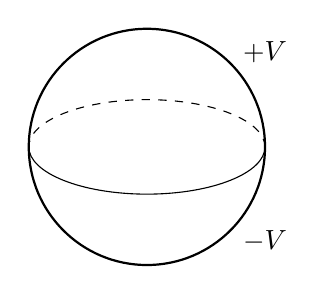
\begin{tikzpicture}[scale=.6]
            \draw[thick](0, 0)circle(2.5);
            \draw[dashed](2.5, 0)arc(0:180:2.5 and 1);
            \draw(-2.5, 0)arc(-180:0:2.5 and 1);
            \node at(2.5, 2){$+V$};
            \node at(2.5, -2){$-V$};
        \end{tikzpicture}
        \captionof{figure}{两半球具有不同电势的导体球}
        \label{fig:2 hemisphere}
    \end{center}
    使用式\eqref{eqn:sphere Laplace solution},
    \begin{align*}
        \Phi(\bm x)&=\frac V{4\pi}\int_0^{2\pi}\biggkh{\int_0^1-\int_{-1}^0}\frac{a(r^2-a^2)}{(r^2+a^2-2ar\cos\gamma)^{3/2}}\d(\cos\theta')\nd\phi'%\\
        % &=\frac{Va(r^2-a^2)}{4\pi}\int_0^{2\pi}\int_0^1\Bigl[(r^2+a^2-2ar\cos\gamma)^{-3/2}-\\
        % &\qqquad(r^2+a^2+2ar\cos\gamma)^{-3/2}\Bigr]\d(\cos\theta')\nd\phi'.
    \end{align*}
    考虑$+z$轴上的电势,取$\theta=0$,则$\cos\gamma=\cos\theta'$,得到 
    \begin{equation}
        \Phi(z)=V\biggfkh{1-\frac{z^2-a^2}{z\sqrt{z^2+a^2}}},
    \end{equation}
    当$z\gg a$时,$\Phi(z)\simeq 3Va^2/2z^2$。
    \tcblower
    为了得到上面积分的表达式,提出$(r^2+a^2)$,
    \begin{align*}
        \Phi(\bm x)&=\frac{Va(r^2-a^2)}{4\pi(r^2+a^2)^{3/2}}\int_0^{2\pi}\int_0^1\Bigl[(1-2\alpha\cos\gamma)^{-3/2}-(1+2\alpha\cos\gamma)^{-3/2}\Bigr]\d(\cos\theta')\nd\phi'
    \end{align*}
    其中$\alpha:=ar/(a^2+r^2)$,进行Taylor展开:
    \[
        (1-2\alpha\cos\gamma)^{-3/2}-(1+2\alpha\cos\gamma)^{-3/2}=6\alpha\cos\gamma+35\alpha^3\cos^3\gamma+\cdots
    \]
    按项积分得到
    \[
        \Phi(\bm x)=\frac{3Va^2}{2r^2}\frac{r^3(r^2-a^2)}{(r^2+a^2)^{5/2}}\cos\theta\biggfkh{1+\frac{35}{24}\frac{a^2r^2}{(r^2+a^2)^2}(3-\cos^2\theta)+\cdots}.
    \]
    若$r\gg a$,则
    \begin{equation}
        \Phi(r,\theta,\phi)=\frac{3Va^2}{2r^2}\biggfkh{\cos\theta-\frac{7a^2}{12r^2}\biggkh{\frac52\cos^3\theta-\frac32\cos\theta}+\cdots}.
    \end{equation}
    对应Legendre多项式$P_1(\cos\theta),P_3(\cos\theta)$。见\exmref{exm:2 hemisphere conductor at different potentials II} 续。
\end{example}
\begin{remark}
    若题目变为两个半导体球,我们也可以写成$(V_1+V_2)/2$的完整孤立导体球与两个$\pm(V_1-V_2)/2$的半导体球的叠加。
\end{remark}

\section{正交函数展开法}
\label{sec:orthogonal functions and expansions}

% \begin{definition}
%     {函数内积}{inner product of funtions}
%     两个实(复)函数$U(\xi),V(\xi)$在区间$(a,b)$上平方可积,可定义内积为
%     \begin{equation}
%         \inp UV:=\int_a^bU\cj(\xi)V(\xi)\rho(\xi)\d\xi.
%     \end{equation}
% \end{definition}

\begin{definition}{正交函数}{orthogonal function}
    一组实(复)函数$U_i(\xi)$在区间$(a,b)$上平方可积,若两两正交(orthogonal):
    \begin{equation}
        \int_a^bU_m^\ast(\xi)U_n(\xi)\d\xi=\delta_{mn}.
    \end{equation}
    则称为正交函数。其中$\delta_{mn}$为Kronecker符号。
\end{definition}
若有一组完备的正交函数集$\{U_i(\xi)\}$,则在区间$(a,b)$上任意平方可积的函数$f(\xi)$均可被展开成正交函数的线性组合
\[
    f(\xi)=\sum_{i=1}^\infty a_iU_i(\xi),\quad a_i:=\int_a^bU_i^\ast(\xi)f(\xi)\d\xi.
\]
即
\[
    f(\xi)=\int_a^b\biggfkh{\sum_{i=1}^\infty U_i^\ast(\xi')U_i(\xi)}f(\xi')\d\xi'.
\]
易得完备(闭合)关系
\begin{equation}
    \sum_{i=1}^\infty U_i^\ast(\xi')U_i(\xi)=\delta(\xi'-\xi).
\end{equation}
\begin{example}{Fourier级数}{Fourier series}
    易证,在区间$(-\pi,\pi)$内,函数集
    \[
        \{1,\sin x,\cos x,\sin 2x,\cos 2x,\ldots\}
    \]
    两两正交。
    % 归一化之
    % \[
    %     \hkh{\frac1{\sqrt{2\pi}},\frac{\sin x}{\sqrt\pi},\frac{\cos x}{\sqrt\pi},\frac{\sin 2x}{\sqrt\pi},\frac{\cos 2x}{\sqrt\pi},\ldots}
    % \]
    % 因此,在$(-\ell/2,\ell/2)$区间内的一组正交函数为
    % \hkh{\frac1{\sqrt\ell},\ldots,\sqrt{\frac2\ell}\sin\biggkh{\frac{2\pi nx}\ell},\enspace\sqrt{\frac2\ell}\cos\biggkh{\frac{2\pi nx}\ell},\ldots}
    因此在$(-\ell/2,\ell/2)$上平方可积的函数$f(x)$可被展开为Fourier级数
    \begin{equation}
        f(x)=\frac{a_0}2+\sum_{n=1}^\infty\biggfkh{a_n\cos\biggkh{\frac{2\pi nx}{\ell}}+b_n\sin\biggkh{\frac{2\pi nx}{\ell}}}.
    \end{equation}
    其中Fourier系数
    \begin{align*}
        a_n&=\frac2\ell\int_{-\ell/2}^{\ell/2}f(x)\cos\biggkh{\frac{2\pi nx}{\ell}}\d x,\\
        b_n&=\frac2\ell\int_{-\ell/2}^{\ell/2}f(x)\sin\biggkh{\frac{2\pi nx}{\ell}}\d x.
    \end{align*}
\end{example}
一般化至二维,对于任意矩形区域$(a,b)\times(c,d)$上平方可积的函数$f(\xi,\eta)$,若可在两个维度分别找到一组正交函数$U_i(\xi),V_j(\eta)$,则$f(\xi,\eta)$可被展开为
\[
    f(\xi,\eta)=\sum_{i=1}^\infty\sum_{j=1}^\infty a_{ij}U_i(\xi)V_j(\eta),
\]
其中 
\[
    a_{ij}=\int_a^b\int_c^dU_i(\xi)V_j(\eta)f(\xi,\eta)\d\eta\nd\xi
\]
\begin{example}{Fourier变换}{Fourier transformation}
    Fourier级数有复变函数的形式
    \[
        f(x)=\frac1{\sqrt\ell}\sum_{n=-\infty}^{+\infty}c_n\e{\i2\pi nx/\ell},\quad c_n=\frac1{\sqrt\ell}\int_{-\ell/2}^{\ell/2}f(x')\e{-\i2\pi nx'/\ell}\d x'.
    \]
    当$\ell\to\infty$时,
    \[
        f(x)=\frac1{2\pi}\int\iti\biggfkh{\int\iti f(x')\e{-\i kx'}\d x'}\e{\i kx}\d k.
    \]
    由此可得$f(x)$的Fourier变换为
    \begin{equation}
        \hat f(k)=\frac1{\sqrt{2\pi}}\int\iti f(x)\e{-\i kx}\d x;
    \end{equation}
    相应的Fourier反变换为
    \begin{equation}
        f(x)=\frac1{\sqrt{2\pi}}\int\iti\hat f(k)\e{\i kx}\d k.
    \end{equation}
    其体现的正交性:
    \[
        \frac1{2\pi}\int\iti\e{\i(k-k')x}\d x=\delta(k-k').
    \]
\end{example}

\subsection{分离变量法}
\label{ssec:separation of variables}

数学物理中的偏微分方程(PED)通常用分离变量的方法来求解。涉及三维Laplacian的方程已知可在11个不同的坐标系中分离\footnote{\href{https://www.researchgate.net/publication/316991519_Morse_and_Feshbach's_Methods_of_Theoretical_Physics_Vol1_Morse_and_Feshbach_1953}{Morse and Feshbach, Methods of Theoretical Physics, Vol.1}}。我们只详细讨论其中的三种:直角坐标、球坐标和柱坐标。

\begin{example}{长方体边界条件下的Laplace方程的解}{solution in cuboid Laplace}
    给定如\figref{fig:cuboid boundary} 所示边界条件,只有$z=c$的边界有电势$V(x,y)$外,其他面电势均为0,求长方体内部电位分布。
    \begin{center}
        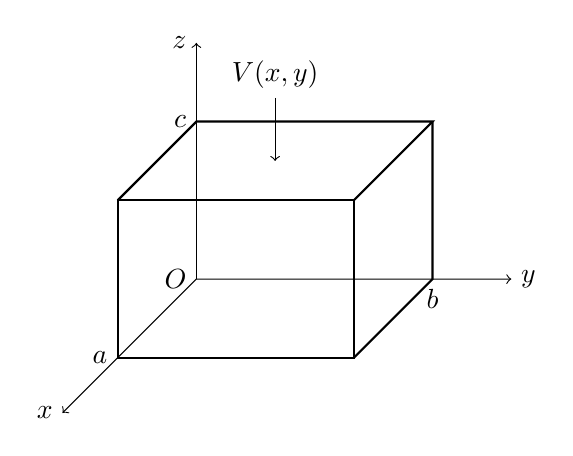
\begin{tikzpicture}
            \draw[thick](0, 0)node[left]{$a$}rectangle(3, 2);
            \draw[thick](0, 2)--(1, 3)node[left]{$c$}--(4, 3)--(3, 2);
            \draw[thick](4, 3)--(4, 1)node[below]{$b$}--(3, 0);
            \draw[<->](5, 1)node[right]{$y$}--(1, 1)node[left]{$O$}--(-.7, -.7)node[left]{$x$};
            \draw[->](1, 1)--(1, 4)node[left]{$z$};
            \draw[->](2, 3.3)node[above]{$V(x,y)$}--(2, 2.5);
        \end{tikzpicture}
        \captionof{figure}{矩形区域边界条件}
        \label{fig:cuboid boundary}
    \end{center}
    直角坐标系下,Laplace方程为
    \[
        \lapla\Phi=\pv[2]\Phi x+\pv[2]\Phi y+\pv[2]\Phi z=0.
    \]
    分离变量,假定解形如$\Phi(x,y,z)=X(x)Y(y)Z(z)$,代入原方程:
    \[
        \frac{X''}X+\frac{Y''}Y+\frac{Z''}Z=0,
    \]
    上式对内部的任意$(x,y,z)$均成立,故
    \[
        X''=-\alpha^2X,\quad Y''=-\beta^2Y,\quad Z''=\gamma^2Z.
    \]
    其中$\gamma^2=\alpha^2+\beta^2$,因为$x=a,\,y=b$处$\Phi=0$,故解为驻波条件:
    \begin{alignat*}{5}
        X_m(x)&=\sin(\alpha_mx),&\qquad\alpha_m&=\frac{m\pi}a,&m&=1,2,3,\ldots\\
        Y_n(y)&=\sin(\beta_ny),&\beta_n&=\frac{n\pi}b,&n&=1,2,3,\ldots\\
        Z_{mn}(z)&=\sinh(\gamma_{mn}z),&\gamma_{mn}&=\pi\sqrt{\frac{m^2}{a^2}+\frac{n^2}{b^2}}.
    \end{alignat*}
    $\Phi$一定可以写成满足Laplace方程的一系列正交函数的线性组合
    \[
        \Phi(x,y,z)=\sum_{m,n}A_{mn}\sin(\alpha_mx)\sin(\beta_ny)\sinh(\gamma_{mn}z).
    \]
    利用$z=c$上的边界条件$\Phi(x,y,c)=V(x,y)$,求得系数
    % V(x,y)=\sum_{m,n}A_{mn}\sin(\alpha_mx)\sin(\beta_ny)\sinh(\gamma_{mn}c).
    \[
        A_{mn}=\frac4{ab\sinh(\gamma_{mn}c)}\int_0^a\int_0^bV(x,y)\sin(\alpha_mx)\sin(\beta_ny)\d y\nd x.
    \]
\end{example}
\begin{remark}
    如果长方体6个面的势都不为零,则我们可以对每个面应用上式,通过6个解的线性叠加得到内部的解。
\end{remark}
% 当内部有电荷分布时,

\subsection{二维边界问题}
\label{ssec:2D boundary problem}

现在我们简单地考虑二维Laplace方程在直角坐标下的分离变量解法。
二维问题假定势与其中一个坐标无关,这通常是一种近似的简化做法,但在一些情况下是很准确的,比如一条均匀的长传输线。

\paragraph{二维直角坐标}

其实就是三维Laplace方程其中一项偏微分为0。

\begin{example}{二维边界条件}{2D boundary condition}
    考虑$0<x<a,\;y>0$的边界,显然$\Phi$与$z$无关:
    \begin{center}
        \begin{tikzpicture}[even odd rule]
            \coordinate (O) at (0, 0);
            \fill[pattern=north east lines](-.5, -.5)rectangle(2.5, 3)(O)rectangle(2, 3);
            \draw[<->](3, 0)node[right]{$x$}--(O)node[left]{$O$}--(0, 3.5)node[left]{$y$};
            \draw[thick](0, 3)--(O)--(2, 0)node[below]{$a$}--(2, 3);
            \draw[<-](1, 0)--(1, 0.5)node[above]{$V(x)$};
        \end{tikzpicture}
        \captionof{figure}{二维边界条件}
    \end{center}
    二维直角坐标Laplace方程为
    \[
        \lap\Phi=\pv[2]\Phi x+\pv[2]\Phi y+\cancel{\pv[2]\Phi z}=0,
    \]
    分离变量$\Phi(x,y)=X(x)Y(y)$,由$\Phi$在$x=0,a$处为0可得
    \[
        X_n(x)=\sin\biggkh{\frac{n\pi x}a},\quad Y_n(y)=\exp\biggkh{-\frac{n\pi y}a},\quad n=1,2,\ldots
    \]
    有形式解
    \begin{equation}
        \Phi(x,y)=\sum_{n=1}^\infty A_n\sin\biggkh{\frac{n\pi x}a}\exp\biggkh{-\frac{n\pi y}a}.
    \end{equation}
    代入边界条件$\Phi(x,0)=V(x)$,
    % \Phi(x,0)=\sum_{n=1}^\infty A_n\sin\biggkh{\frac{n\pi x}a}=V(x),
    得到系数
    \[
        A_n=\frac2a\int_0^aV(x)\sin\biggkh{\frac{n\pi x}a}\d x.
    \]
\end{example}
\paragraph{二维极坐标}
二维极坐标Laplace方程为柱坐标Laplace中$z$坐标偏微分为0:
\begin{equation}
    \lap\Phi=\frac1\rho\pp\rho\biggkh{\rho\pv\Phi\rho}+\frac1{\rho^2}\pv[2]\Phi\phi+\cancel{\pv[2]\Phi z}%=\pv[2]\Phi\rho+\frac1\rho\pv\Phi\rho+\frac1{\rho^2}\pv[2]\Phi\phi
    =0.
\end{equation}
分离变量$\Phi(\rho,\phi)=R(\rho)\Psi(\phi)$,得到
\[
    \rho^2R''+\rho R'+\frac{\Psi''}\Psi R=0.
\]
若$\phi$的范围是任意的,则由周期条件
\[
    \begin{cases}
        \Psi(\phi+2\pi)=\Psi(\phi),\\
        \Psi'(\phi+2\pi)=\Psi'(\phi)
    \end{cases}\implies
    \Psi_n(\phi)=a_n\cos(n\phi)+b_n\sin(n\phi),
    \enspace n=0,1,2,\ldots
\]
可得$\Psi_n''/\Psi_n=n^2$,
继而$R(\rho)$满足Euler方程,
% 做变量替换$u(t)=R(\e t)$,
% \[
%     u''-n^2u=0\implies u=
%     \begin{cases}
%         c_0+d_0t,&n=0\\
%         c_n\e{nt}+d_n\e{-nt},&n\geqslant 1
%     \end{cases}
% \]
可得
\[
    R_n(\rho)=
    \begin{cases}
        c_0+d_0\ln\rho,&n=0\\
        c_n\rho^n+d_n\rho^{-n},&n\geqslant 1
    \end{cases}
\]
故
\begin{equation}
    \Phi(\rho,\phi)=c_0+d_0\ln\rho+\sum_{n=1}^{\infty}(a_n\cos(n\phi)+b_n\sin(n\phi))(c_n\rho^n+d_n\rho^{-n}).
\end{equation}
若区域包含原点,则要求$d_n\equiv 0$。
\begin{example}{二维拐角内和沿棱边的电场与电荷密度}{field and charge density in 2D Corners and along edges}
    \begin{center}
        \begin{tikzpicture}
            \coordinate (o) at (0, 0);
            \coordinate (p) at (4, 1);
            \coordinate (a) at (5, 0);
            \coordinate (b) at (3, 4);
            \fill[pattern=north east lines](2.3, 4)--(b)--(o)--(a)--(5, -.4)--(-.8, -.4);
            \draw[thick](b)--(o)node[left]{$O$}--(a);
            \draw[dashed](o)--(p)node[right]{$P$}node[midway, above, sloped]{$\rho$};
            \fill(p)circle(.05);
            \pic[draw, angle radius=20, angle eccentricity=1.5, "$\beta$"]{angle=a--o--b};
            \pic[draw, angle radius=40, angle eccentricity=1.25, "$\phi$"]{angle=a--o--p};
        \end{tikzpicture}
        \captionof{figure}{极坐标}
    \end{center}
    由边界条件,在$\phi=0,\beta$时$\Phi=V$可得
    \begin{equation}
        \Phi(\rho,\phi)=V+\sum_{n=1}^\infty a_n\rho^{n\pi/\beta}\sin\biggkh{\frac{n\pi\phi}\beta}.
    \end{equation}
    $\rho\to0$时,忽略高阶项
    \[
        \Phi\simeq V+a_1\rho^{\pi/\beta}\sin\biggkh{\frac{\pi\phi}\beta}.
    \]
    电场 
    \begin{equation}
        \begin{cases}
            E_\rho=-\pv\Phi\rho\simeq-\frac{\pi a_1}\beta\rho^{\pi/\beta-1}\sin\biggkh{\frac{\pi\phi}\beta}.\\
            E_\phi=-\frac1\rho\pv\Phi\phi\simeq-\frac{\pi a_1}\beta\rho^{\pi/\beta-1}\cos\biggkh{\frac{\pi\phi}\beta}
        \end{cases}
    \end{equation}
    边界感应电荷密度
    \begin{equation}
        \sigma(\rho)=\varepsilon_0E_\phi(\rho,0)\simeq-\frac{\varepsilon_0\pi a_1}\beta\rho^{\pi/\beta-1}.
    \end{equation}
    当$\beta>\pi$时,$\sigma$在$\rho\to0$有奇点。这便是尖端放电现象的解释。
\end{example}

\sectionstar{有限元分析法}
\label{sec:finite element analysis}

有限元分析法(finite element analysis, FEA)是一种数值计算方法。具体可见电磁场数值计算课程笔记。此处略。

% \par\noindent\rule{\textwidth}{0.5pt}
\clearpage

\paragraph{第二部分}
这一部分继续讨论静电学中的边值问题,主要内容分为四节:
\begin{itemize}
    \item \secref{sec:laplace equation in spherical coordinate}和\secref{sec:laplace equation in cylindrical coordinate}讲在球坐标和柱坐标中用分离变量法求解Laplace方程,并介绍了Legendre多项式、球谐函数、Bessel函数等特殊函数的性质;
    \item \secref{sec:Green expansion solve Poisson}内容为在球坐标系和柱坐标系中应用Green函数展开法求解Poisson方程;
    \item \secref{sec:mixed boundary condition}举例讨论了混合边界条件下的边值问题。
\end{itemize}
一些数学内容(如特殊函数的级数表达式、收敛问题,以及各种完备性的证明等)可见数学物理方法笔记,此处不作为重点讲述,故省略。

%值得一提的是,本章内容大多和MMP(数学物理方法,Methods of Mathematical Physics)挂钩,所以一些数学计算的过程(如特殊函数的级数表达式、收敛问题,以及各种完备性的证明等……)被我省略掉了,具体内容可以参考:

\section{球坐标系中的正交函数}
\label{sec:laplace equation in spherical coordinate}

球坐标系$(r,\theta,\phi)$中Laplace方程可以写成
\begin{equation}
    \label{eqn:Laplace in spherical}
    \lap\Phi=\frac1{r^2}\pp r\biggkh{r^2\pv\Phi r}+\frac1{r^2\sin\theta}\pp\theta\biggkh{\sin\theta\pv\Phi\theta}+\frac1{r^2\sin^2\theta}\pv[2]\Phi\phi=0.
\end{equation}
分离变量$\Phi(r,\theta,\phi)=R(r)P(\theta)Q(\phi)$,得到 
\[
    \begin{cases}
        \dd r\biggkh{r^2\dv Rr}-\ell(\ell+1)R=0,\\
        \frac1{\sin\theta}\dd\theta\biggkh{\sin\theta\dv P\theta}+\biggfkh{\ell(\ell+1)-\frac{m^2}{\sin^2\theta}}P=0,\\
        \frac1Q\dv[2]Q\phi=-m^2.
    \end{cases}
\]
可直接解得$R,Q$
\begin{align}
    R_\ell(r)&=Ar^\ell+Br^{-(\ell+1)},\\
    Q_m(\phi)&=\e{\pm\i m\phi},\quad m=0,\pm 1,\pm 2,\ldots
\end{align}

\subsection{Legendre多项式}
\label{ssec:Legendre polynomial}

$P(\theta)$经常通过$x=\cos\theta$代换,得到广义(generalized) Legendre方程:
\begin{equation}
    \label{eqn:general Legendre}
    \dd x\biggfkh{(1-x^2)\dv Px}+\biggfkh{\ell(\ell+1)-\frac{m^2}{1-x^2}}P=0.
\end{equation}
考虑$m=0$的情形,得到Legendre方程:
\begin{equation}
    \label{eqn:Legendre}
    \dd x\biggfkh{(1-x)^2\dv Px}+\ell(\ell+1)P=0.
\end{equation}
采用级数解,设
\[
    P(x)=x^\alpha\sum_{j=0}^\infty a_jx^j.
\]
$\alpha$是待定系数,从而 
\[
    \sum_{j=0}^\infty(\alpha+j)(\alpha+j-1)a_j x^{\alpha+j-2}-\sum_{j=0}^\infty\bigfkh{(\alpha+j)(\alpha+j+1)-\ell(\ell+1)}a_jx_{\alpha+j}=0.
\]
解得
\[
    \begin{cases}
        a_0\alpha(\alpha-1)=0,&j=0\\
        a_1\alpha(\alpha+1)=0,&j=1\\
        a_{j+2}=\frac{(\alpha+j)(\alpha+j+1)-\ell(\ell+1)}{(\alpha+j+1)(\alpha+j+2)}a_j,&j\geqslant 0
    \end{cases}
\]
对初始条件分情况讨论:
\begin{compactitem}
	\item $a_0=a_1=0$,解$P\equiv 0$是平凡的;
	\item $a_0=0,\enspace a_1\neq 0$,展开式事实上与$a_0\neq 0,\enspace a_1=0$等价:
	\[
        P(x)=x^\alpha(a_1x+a_3x^3+\cdots)=x^{\alpha+1}(a_1+a_3x^2+\cdots);
    \]
	\item $a_0\neq 0,\enspace a_1\neq 0$,由递推关系知,级数会在$x=\pm 1$发散。
\end{compactitem}
综上,我们最终选取$a_0\neq 0,\enspace a_1=0$,从而$\alpha(\alpha-1)=0$,
\[
    P(x)=\begin{cases}
        a_0+a_2x^2+a_4x^4+\cdots,&\alpha=0\\
        a_0x+a_2x^3+a_4x^5+\cdots,&\alpha=1
    \end{cases}
\]
这个级数在$|x|<1$时当然收敛,但在$x=\pm 1$时会发散,除非级数在某一项截断(即此项之后的系数均为0)。考察递推关系:
\[
    a_{j+2}=\begin{cases}
        \frac{j(j+1)-\ell(\ell+1)}{(j+1)(j+2)}a_j,&\alpha=0\\[2ex]
        \frac{(j+1)(j+2)-\ell(\ell+1)}{(j+2)(j+3)}a_j,&\alpha=1
    \end{cases}
\]
因此,收敛性要求$\ell=0,1,2,\ldots$
\begin{example}{前几个Legendre多项式}{Legendre polynomial}
    \begin{center}
        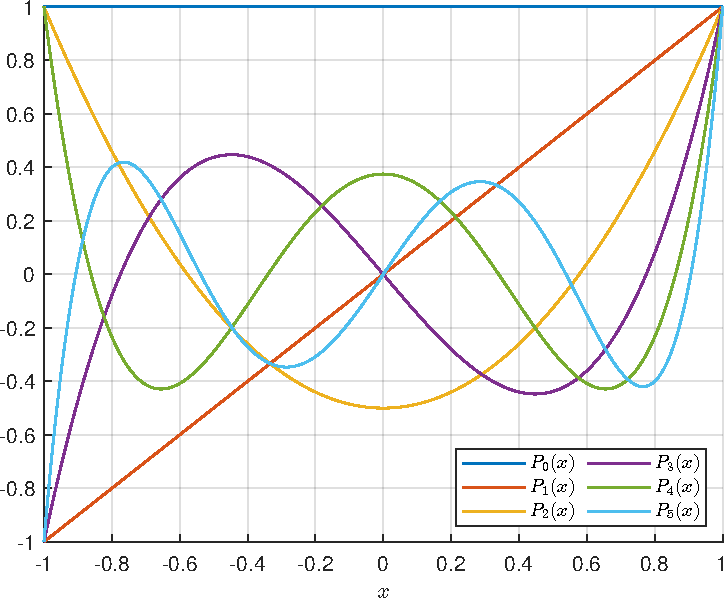
\includegraphics[width=7cm]{graphs/Legendre.pdf}
        \captionof{figure}{前几个Legendre多项式}
    \end{center}
    \begin{equation*}
        \begin{aligned}
            P_0&=1,&\qquad P_2&=\frac12(3x^2-1),&\quad P_4&=\frac18(35x^4-30x^2+3),\\
            P_1&=x,&P_3&=\frac12(5x^3-3x),&P_5&=\frac18(63x^5-70x^3+15x).
        \end{aligned}
    \end{equation*}
\end{example}
\begin{theorem}{Rodrigues公式}{Rodrigues' formula}
    Legendre多项式可被表示为
    \begin{equation}
        \label{eqn:Rodrigues}
        P_\ell(x)=\frac1{2^\ell\ell!}\dd[\ell]x(x^2-1)^\ell.
    \end{equation}
\end{theorem}
\begin{theorem}
    {Legendre多项式的正交性}{}
    Legendre多项式是正交的
    \[
        \int_{-1}^1P_\ell(x)P_{\ell'}(x)\d x=\frac2{2\ell+1}\vd_{\ell\ell'}.
    \]
    因此任意$[-1,1]$上的函数$f(x)$均可被展开为Legendre级数
    \[
        f(x)=\sum_{\ell=0}^\infty A_\ell P_\ell(x),\quad A_\ell=\frac{2\ell+1}2\int_{-1}^1f(x)P_\ell(x)\d x.
    \]
\end{theorem}
\begin{theorem}{Legendre多项式的递推关系}{recurrence relation among Legendre polynomial}
    可直接从Rodrigues公式和Legendre方程得到:
    \begin{gather}
        \label{eqn:Legendre 1 recurrence}
        P'_{\ell+1}-P'_{\ell-1}-(2\ell+1)P_\ell=0,\\
        (\ell+1)P_{\ell+1}-(2\ell+1)xP_\ell+\ell P_{\ell+1}=0,\\
        \notag
        P'_{\ell+1}-xP'_\ell-\ell(\ell+1)P_\ell=0,\\
        \notag
        (x^2-1)P'_\ell-\ell xP_\ell+\ell P_{\ell-1}=0.
    \end{gather}
\end{theorem}
综上,对于方位角$\phi$对称的Laplace方程\eqref{eqn:Laplace in spherical},$m=0$,其解为
\begin{equation}
    \label{eqn:Phi(r, theta)}
    \Phi(r,\theta)=\sum_{\ell=0}^\infty\bigfkh{A_\ell r^\ell+B_\ell r^{-(\ell+1)}}P_\ell(\cos\theta).
\end{equation}
若区域包含原点,则要求$B_\ell\equiv 0$。
\begin{example}{两半球具有不同电势的导体球(续)}{2 hemisphere conductor at different potentials II}
    接\exmref{exm:2 hemisphere conductor at different potentials},边界条件为
    \[
        \Phi(a,\theta)=V(\theta)=
        \begin{cases}
            +V,&0\leqslant\theta<\pi/2\\
            -V,&\pi/2<\theta\leqslant\pi
        \end{cases}
    \]
    因此解具有\eqref{eqn:Phi(r, theta)}的形式,而系数满足
    \[
        A_\ell a^\ell=\frac{2\ell+1}2\int_0^\pi V(\theta)P_\ell(\cos\theta)\sin\theta\d\theta
    \]
    由于$P_\ell$与$\ell$具有相同的奇偶性,因此只有$\ell$为奇数的项不为0,进而由\eqref{eqn:Rodrigues}计算
    得$r<a$时,
    \[
        \Phi=V\biggfkh{\frac32\frac raP_1(\cos\theta)-\frac78\Bigkh{\frac ra}^3P_3(\cos\theta)+\frac{11}{16}\Bigkh{\frac ra}^5P_5(\cos\theta)+\cdots}.
    \]
    \tcblower
    球外电势,$r>a$,$A_\ell\equiv 0$。只需将$(r/a)^\ell$替换为$(a/r)^{\ell+1}$即可。
\end{example}
由于注意到$z$轴上$\theta=0,\enspace P_\ell(\cos\theta)=1$,因此另一种求解方法是先求出$z$轴上的电势,再在级数的项中添加对应的$P_\ell(\cos\theta)$。
% 下面是此方法的两个例子。

\begin{example}{点电荷电势}{point charge potential}
    $\bm x'$处的单位点电荷在$\bm x$的产生的电势为
    \begin{equation}
        \label{eqn:1/|x-x'|}
        \frac1{|\bm x-\bm x'|}=\frac1{r_>}\sum_{\ell=0}^\infty\biggkh{\frac{r_<}{r_>}}^\ell P_\ell(\cos\gamma).
    \end{equation}
    其中$r_<:=\min(x,x'),\enspace r_>:=\max(x,x')$,$\gamma$是$\bm x,\bm x'$夹角。
\end{example}
% \begin{example}{带电圆环的电势}{charged ring}
    
% \end{example}
\begin{example}{锥形孔内尖端附近的电场特性}{field near the tip of the conical hole}
    如图所示的锥形孔边界,求其尖端附近的电场特性。
    \begin{center}
        \begin{tikzpicture}
            \coordinate (o) at (0, 0);
            \coordinate (z) at (0, 5);
            \coordinate (a) at (3, 5);
            \coordinate (b) at (-3, 5);
            \coordinate (p) at (1, 4);
            \fill[pattern=north east lines](b)--(o)--(a)--(3, 4.5)--(0, -.5)--(-3, 4.5);
            \draw[thick](a)--(o)--(b);
            \draw[dashed](z)--(o)--(p);
            \draw[dashed](0, 3)ellipse(1.75 and .5);
            \fill(p)circle(.05)node[right]{$P$};
            \pic[draw, angle radius=30, angle eccentricity=1.25, "$\beta$"]{angle=z--o--b};
            \pic[draw, angle radius=50, angle eccentricity=1.25, "$\theta$"]{angle=p--o--z};
        \end{tikzpicture}
        \captionof{figure}{锥形孔}
    \end{center}
    在$\theta=0$附近展开,设$\xi:=(1-\cos\theta)/2$,则 
    \[
        \dd\xi\biggfkh{\xi(1-\xi)\dv P\xi}+\nu(\nu+1)P=0.
    \]
    注意此式与Legendre方程\eqref{eqn:Legendre}的区别。设级数解,有
    \[
        a_{j+1}=\frac{(j-\nu)(j+\nu+1)}{(j+1)^2}a_j.
    \]
    得到Legendre函数的一般表达式,这是Legendre多项式的推广:
    \[
        P_\nu(\xi)=1+(-\nu)(\nu+1)\xi+\frac{(-\nu)(-\nu+1)(\nu+1)(\nu+2)}{(2!)^2}\xi^2+\cdots.
    \]
    形式解
    \[
        \Phi=Ar^\nu P_\nu(\cos\theta).
    \]
    边界条件$P_\nu(\cos\beta)=0$,可解得$\nu=\nu_k,\enspace k=1,2,\ldots$
    \[
        \Phi(r,\theta)=\sum_{k=1}^\infty A_kr^{\nu_k}P_{\nu_k}(\cos\theta).
    \]
    $r\to 0$时,考虑第一项$\Phi\simeq Ar^\nu P_\nu(\cos\theta)$,电场
    \[
        \begin{cases}
            E_r=-\pv\Phi r\simeq-\nu Ar^{\nu-1}P_\nu(\cos\theta),\\[1ex]
            E_\theta=-\frac1r\pv\Phi\theta\simeq Ar^{\nu-1}\sin\theta P'_\nu(\cos\theta).
        \end{cases}
    \]
    表面电荷密度
    \[
        \sigma_r=-\varepsilon_0E_\theta|_{\theta=\beta}\simeq-\varepsilon_0Ar^{\nu-1}\sin\beta P_\nu'(\cos\beta).
    \]
\end{example}

\subsection{连带Legendre函数、球谐函数}
\label{ssec:associated Legendre function and spherical harmonics}

考虑式\eqref{eqn:general Legendre} $m\neq 0$的情形,
% $\ell=0,1,2,\ldots$且$m=-\ell,-\ell+1,\ldots,\ell$,
为了使解在$[-1,1]$收敛,略去推导过程,要求:
\[
    \ell=0,1,2,\ldots,\quad m=-\ell,-\ell+1,\ldots,\ell.
\]
解是连带(associated) Legendre函数:
\begin{equation}
    P_\ell^m(x)=(-)^m(1-x^2)^{m/2}\dd[m]xP_\ell(x),
\end{equation}
上式默认$m>0$,因为$P_\ell^{-m}$和$P_\ell^m$是线性相关的:
\[
    P_\ell^{-m}(x)=(-)^m\frac{(\ell-m)!}{(\ell+m)!}P_\ell^m(x).
\]
有正交关系:
\begin{align*}
    \int_{-1}^1P_\ell^m(x)P_{\ell'}^m(x)\d x&=\frac2{2\ell+1}\frac{(\ell-m)!}{(\ell+m)!}\vd_{\ell\ell'};\\
    \int_{-1}^1P_\ell^m(x)P_\ell^{m'}(x)\frac{\d x}{1-x^2}&=\frac1m\frac{(\ell+m)!}{(\ell-m)!}\vd_{mm'}.
\end{align*}
由此得到球谐函数(spherical harmonics fucntion):
\begin{equation}
    Y_{\ell m}(\theta,\phi)=\sqrt{\frac{2\ell+1}{4\pi}\frac{(\ell-m)!}{(\ell+m)!}}P_\ell^m(\cos\theta)\e{\i m\phi}.
\end{equation}
满足方程
\[
    \frac1{\sin\theta}\pp\theta\biggkh{\sin\theta\pv Y\theta}+\frac1{\sin^2\theta}\pv[2]Y\phi+\ell(\ell+1)Y=0,
\]
球谐函数自然是正交函数:
\[
    \oint Y_{\ell m}^\ast Y_{\ell'm'}\d\Omega=\int_0^{2\pi}\int_0^\pi Y_{\ell m}^\ast(\theta,\phi) Y_{\ell'm'}(\theta,\phi)\sin\theta\d\theta\nd\phi=\delta_{\ell\ell'}\vd_{mm'}.
\]
\begin{equation}
    \sum_{\ell=0}^\infty\sum_{m=-\ell}^\ell Y_{\ell m}^*(\theta,\phi)Y_{\ell m}(\theta,\phi)=\delta(\phi-\phi')\delta(\cos\theta-\cos\theta').
\end{equation}
这样我们便得到了球坐标系下Laplace方程\eqref{eqn:Laplace in spherical}的通解
\begin{equation}
    \Phi(r,\theta,\phi)=\sum_{\ell=0}^\infty\sum_{m=-\ell}^\ell\bigfkh{A_{\ell m}r^\ell+B_{\ell m}r^{-(\ell+1)}}Y_{\ell m}(\theta,\phi).
\end{equation}
由$P_\ell(\cos\gamma)$的球谐函数展开式及\eqref{eqn:1/|x-x'|},点电荷之间电势的球谐函数展开
\begin{equation}
    \label{eqn:1/|x-x'|=YY}
    \frac1{|\bm x-\bm x'|}=\frac{4\pi}{r_>}\sum_{\ell=0}^\infty\biggfkh{\frac1{2\ell+1}\biggkh{\frac{r_<}{r_>}}^\ell\cdot\sum_{m=-\ell}^\ell Y^\ast_{\ell m}(\theta',\phi')Y_{\ell m}(\theta,\phi)}.
\end{equation}

\section{柱坐标系中的正交函数}
\label{sec:laplace equation in cylindrical coordinate}

柱坐标系$(\rho,\phi,z)$,Laplace方程可以写成
\begin{equation}
    \label{eqn:Laplace in cylinder}
    \frac1\rho\pp\rho\biggkh{\rho\pv\Phi\rho}+\frac1{\rho^2}\pv[2]\Phi\phi+\pv[2]\Phi z=0.
\end{equation}
分离变量$\Phi(\rho,\phi,z)=R(\rho)Q(\phi)Z(z)$,得到 
\[
    \begin{cases}
        \dv[2]R\rho+\frac1\rho\dv R\rho+\biggkh{k^2-\frac{\nu^2}{\rho^2}}R=0,\\[1ex]
        \dv[2]Q\phi+\nu^2Q=0,\\[1ex]
        \dv[2]Zz-k^2Z=0.
    \end{cases}
\]
可直接解得$Q,Z$
\begin{alignat}{2}
    Q_\nu(\phi)&=\e{\pm\i\nu\phi},\quad&\nu&=0,\pm 1,\pm 2,\ldots\\
    Z_k(z)&=\e{\pm kz},&k&>0
\end{alignat}

\subsection{Bessel函数}
\label{ssec:Bessel functions}

设$x=k\rho$,得到Bessel方程
\begin{equation}
    \label{eqn:Bessel eqn}
    \dv[2]Rx+\frac1x\dv Rx+\biggkh{1-\frac{\nu^2}{x^2}}R=0.
\end{equation}
采用级数解,设 
\[
    R(x)=x^\alpha\sum_{j=0}^\infty a_jx^j.
\]
解得
\[
    \begin{cases}
        \alpha^2=\nu^2,&j=0\\
        a_1\bigfkh{(\alpha+1)^2-\nu^2}=0,&j=1\\
        a_{j-2}=\bigfkh{\nu^2-(j+\alpha)^2}a_j,&j\geqslant 2
    \end{cases}
\]
故$\alpha=\pm\nu,\enspace a_1=0$,从而
\[
    a_{2j}=-\frac1{4j(j+\alpha)}a_{2j-2},\quad j=1,2,\ldots
\]
选取\footnote{$\nu$可以不是整数,此时阶乘$\nu!$推广为$\Gamma(\nu+1)$。}
\[
    \alpha=\nu,\enspace a_0=\frac1{2^\nu\nu!}.
\]
解得(第一类) Bessel函数
\begin{equation}
    J_\nu(x)=\sum_{j=0}^\infty\frac{(-)^j}{j!(j+\nu)!}\Bigkh{\frac x2}^{2j+\nu},
\end{equation}
当$\nu$不为整数时,$J_{-\nu}$和$J_\nu$是线性无关的,可作为Bessel方程的解系;但当$\nu$为整数时,二者线性相关:
\[
    J_{-\nu}(x)=(-)^\nu J_\nu(x),
\]
为了得到线性无关的另一解,定义Neumann函数(第二类Bessel函数)
\begin{equation}
    Y_\nu(x):=\frac{J_\nu(x)\cos(\nu\pi)-J_{-\nu}(x)}{\sin(\nu\pi)}.
\end{equation}
当$\nu$为整数时,$Y_\nu(x)$的值定义为上式$\nu$趋近于该整数的极限(即可去间断点)。可以证明,$J_\nu,Y_\nu$线性无关。

\begin{figure}[!htp]
    \centering
    \subcaptionbox{第一类Bessel函数\label{fig:bessel J function}}
      {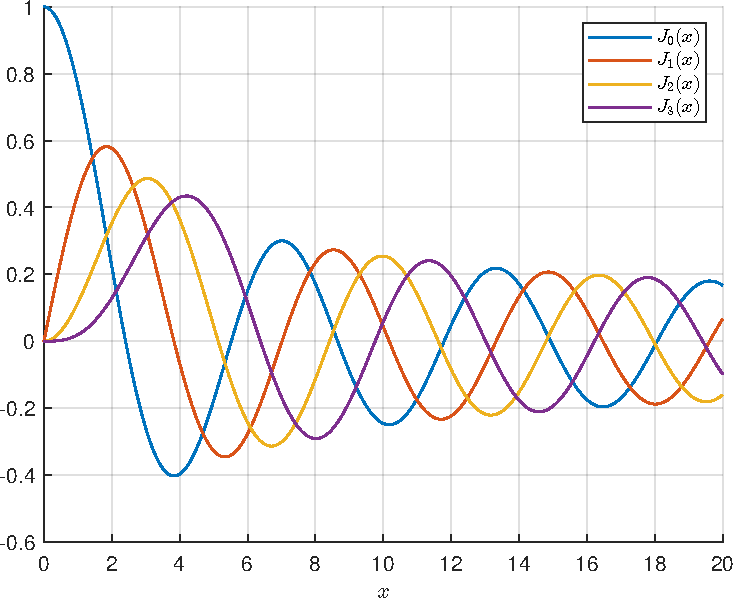
\includegraphics[width=0.45\linewidth]{graphs/BesselJ.pdf}}
    \subcaptionbox{第二类Bessel函数\label{fig:bessel Y function}}
      {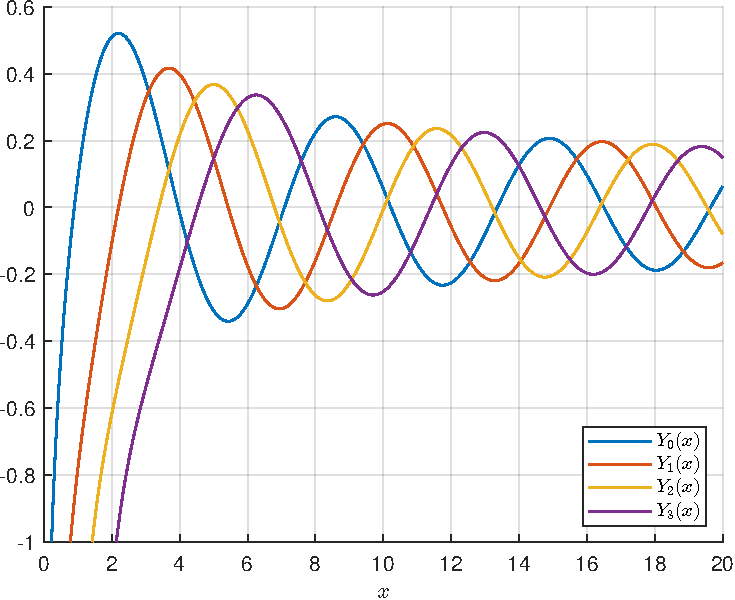
\includegraphics[width=0.45\linewidth]{graphs/BesselY.pdf}}
    \caption{前几个Bessel函数}
    \label{fig:Bessel function}
\end{figure}

Bessel方程的另一对重要线性无关解是Hankel函数(第三类Bessel函数)
\begin{equation}
    H_\nu^\pm(x)=J_\nu(x)\pm\i Y_\nu(x).
\end{equation}
三类Bessel函数均满足形如下面的递推公式
\begin{align*}
    \Omega_{\nu-1}+\Omega_{\nu+1}&=\frac{2\nu}x\Omega_\nu,\\
    \Omega_{\nu-1}-\Omega_{\nu+1}&=2\Omega'_\nu.
\end{align*}


\begin{example}{Bessel函数的渐进性}{limit of Bessel function}
    $x\to 0$时, 
    \begin{align*}
        J_\nu(x)&\simeq\frac1{\nu!}\Bigkh{\frac x2}^\nu,\quad\\
        Y_\nu(x)&\simeq
        \begin{cases}
            \frac2\pi\Bigfkh{\ln\Bigkh{\frac x2}+\gamma},&\nu=0\\[1ex]
            -\frac{(\nu-1)!}\pi\Bigkh{\frac x2}^{-\nu}+\frac{\cot(\nu\pi)}{\nu!}\Bigkh{\frac x2}^\nu,&\nu\neq 0
        \end{cases}
    \end{align*}
    其中$\gamma$是Euler-Mascheroni常数
    \[
        \gamma:=\lim_{n\to\infty}\biggkh{-\ln n+\sum_{k=1}^n\frac1k}=\num{0.5772156649}\ldots.
    \]
    \tcblower
    $x\to\infty$时, 
    \begin{align*}
        J_\nu(x)&\simeq\sqrt{\frac2{\pi x}}\cos\biggkh{x-\frac{\nu\pi}2-\frac\pi{4}},\\
        Y_\nu(x)&\simeq\sqrt{\frac2{\pi x}}\sin\biggkh{x-\frac{\nu\pi}2-\frac\pi{4}}.
    \end{align*}
\end{example}
若将$k$替换为$\i k$,便会得到修正(modified) Bessel方程
\[
    \dv[2]Rx+\frac1x\dv Rx-\biggkh{1+\frac{\nu^2}{x^2}}R=0.
\]
修正Bessel函数只是纯虚数参数的Bessel函数
\[
    I_\nu(x)=\i^{-\nu}J_\nu(\i x),\quad K_\nu(x)=\i^{\nu+1}\frac\pi 2H_\nu^+(\i x).
\]
\begin{theorem}{Bessel函数的正交性}{}
    令$x_{\nu n}$是$J_\nu(x)$的第$n$个零点,则
    \begin{equation}
        \int_0^a J_\nu\Bigkh{x_{\nu n}\frac\rho a}J_\nu\Bigkh{x_{\nu n'}\frac\rho a}\rho\d\rho=\frac{a^2}2J_{\nu+1}^2(x_{\nu n})\vd_{nn'}.
    \end{equation}
    因此$[0,a]$上的函数$f(\rho)$均可被展开为Bessel级数
    \[
        f(\rho)=\sum_{n=1}^\infty A_{\nu n}J_\nu\biggkh{x_{\nu n}\frac\rho a},
    \]
    系数 
    \[
        A_{\nu n}=\frac2{a^2J_{\nu+1}^2(x_{\nu n})}\int_0^af(\rho)J_\nu\biggkh{x_{\nu n}\frac\rho a}\rho\d\rho.
    \]
\end{theorem}
%\prf $n\neq n'$时,由正交条件知,积分为0;$n=n'$证明略。\qed

\begin{example}{圆柱体内电势分布}{potential inside cylinder}
    如下图,圆柱体除顶面外其余面电势均为0.
    \begin{center}
        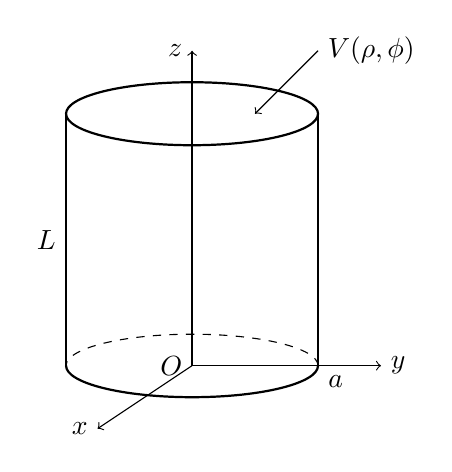
\begin{tikzpicture}[scale=.8]
            \draw[<->](0, 5)node[left]{$z$}--(0, 0)node[left]{$O$}--(3, 0)node[right]{$y$};
            \draw[->](0, 0)--(-1.5, -1)node[left]{$x$};
            \draw[dashed](2, 0)arc(0:180:2 and .5);
            \draw[thick](-2, 0)arc(-180:0:2 and .5);
            \draw[thick](0, 4)ellipse(2 and .5);
            \draw[thick](2, 0)node[below right]{$a$}--(2, 4);
            \draw[thick](-2, 0)--(-2, 4)node[midway, left]{$L$};
            \draw[<-](1, 4)--(2, 5)node[right]{$V(\rho,\phi)$};
        \end{tikzpicture}
        \captionof{figure}{圆柱形边界条件}
    \end{center}
    由边界条件可知,
    \iffalse :
    \begin{align*}
        Q(\phi)&=A\sin m\phi+B\cos m\phi,\\
        Z(z)&=\sinh kz.
    \end{align*}
    \fi
    电势有形式解
    \[
        \Phi(\rho,\phi,z)=\sum_{m=0}^\infty\sum_{n=1}^\infty J_m(k_{mn}\rho)\sinh(k_{mn}z)(A_{mn}\sin(m\phi)+B_{mn}\cos(m\phi)).
    \]
    $z=L$处边界条件$\Phi(\rho,\phi,L)=V(\rho,\phi)$,可得系数
    \[
        \begin{cases}
            A_{mn}=\frac{2\csch(k_{mn}L)}{\pi a^2J_{m+1}^2(k_{mn}a)}\int_0^{2\pi}\int_0^aV(\rho,\phi)J_m(k_{mn}\rho)\sin(m\phi)\rho\d\rho\nd\phi\\
            B_{mn}=\frac{2\csch(k_{mn}L)}{\pi a^2J_{m+1}^2(k_{mn}a)}\int_0^{2\pi}\int_0^aV(\rho,\phi)J_m(k_{mn}\rho)\cos(m\phi)\rho\d\rho\nd\phi
        \end{cases}
    \]
\end{example}

\section{Green函数展开法解Poisson方程}
\label{sec:Green expansion solve Poisson}

在\secref{ssec:Green solve Poisson}中,我们介绍了Green函数方法。对于三种不同边界条件下的Poisson方程,我们给出了\eqref{eqn:Dirichlet Green}和\eqref{eqn:Neumann Green}的通解形式。在本章前面,我们用正交函数解了球坐标和柱坐标下的Laplace方程。在本节中,我们将重点讨论使用Green函数求解带有Dirichlet边界的Poisson方程。

由式\eqref{eqn:Dirichlet Green},带Dirichlet边界条件的Poisson方程的形式解为:
\[
    \Phi(\bm x)=\frac1{4\pi\varepsilon_0}\int_V\rho(\bm x')G(\bm x,\bm x')\d v'-\frac1{4\pi}\oint_{\p V}\Phi(\bm x')\pv G{n'}\d a';
\]
因此有必要确定满足边界条件的Green函数$G(\bm x,\bm x')$。

\subsection{球坐标系下Green函数的展开}
\label{ssec:Green expansion in spherical coordinate}

对于球面边界条件,我们通常选择球坐标。然后,将Green函数表示为与所讨论的坐标相适应的函数的一系列乘积就很方便了。

事实上,根据我们所介绍的,我们可以简单地得到球坐标下Green函数的展开式。由式\eqref{eqn:1/|x-x'|=YY},
\[
    \frac1{|\bm x-\bm x'|}=4\pi\sum_{\ell=0}^\infty\biggfkh{\frac1{2\ell+1}\frac{r_<^\ell}{r_>^{\ell+1}}\cdot\sum_{m=-\ell}^\ell Y^\ast_{\ell m}(\theta',\phi')Y_{\ell m}(\theta,\phi)}.
\]
我们希望得到适用于在$r = a$处具有球面边界的外部问题的Green函数的类似展开。由式\eqref{eqn:sphere Green function}易得:
\[
    G(\bm x,\bm x')=\frac1{|\bm x-\bm x'|}-\frac a{x'}\frac1{|\bm x-\bm x''|},\quad\bm x''=\Bigkh{\frac{a}{x'}}^2\bm x'.
\]
对式\eqref{eqn:sphere Green function}中的两项展开\eqref{eqn:1/|x-x'|=YY},得到
\begin{equation}
    \label{eqn:Green YY}
    G(\bm x,\bm x')=4\pi\sum_{\ell=0}^\infty\biggfkh{\frac1{2\ell+1}\frac1{r_>^{\ell+1}}\biggkh{r_<^\ell-\frac{a^{2\ell+1}}{r_<^{\ell+1}}}\sum_{m=-\ell}^\ell Y_{\ell m}^\ast(\theta',\phi')Y_{\ell m}(\theta,\phi)}.
\end{equation}
其中$r_>=\max(r,r'),\enspace r_<=\min(r,r')$。%,展开可得
\iffalse
\[
    \frac{r_<^\ell}{r_>^{\ell+1}}-\frac1a\biggkh{\frac{a^2}{rr'}}^{\ell+1}=
    \frac1{r_>^{\ell+1}}\biggkh{r_<^\ell-\frac{a^{2\ell+1}}{r_<^{\ell+1}}}
    \begin{cases}
        \frac1{r'^{\ell+1}}\biggkh{r^\ell-\frac{a^{2\ell+1}}{r^{\ell+1}}},&r<r'\\
        \biggkh{r'^\ell-\frac{a^{2\ell+1}}{r'^{\ell+1}}}\frac1{r^{\ell+1}},&r>r'
    \end{cases}
\]
\fi
\paragraph{一般展开式}
现在我们从基本原理开始,来系统地构建这种展开。有%Dirichlet势问题的Green函数满足:
\[
    \lapla G(\bm x,\bm x')=-4\pi\vd(\bm x,\bm x').
\]
且$G(\bm x,\bm x')|_{\p V}=0$。
对于球坐标,$\delta$函数可以写成
\begin{align*}
    \delta(\bm x,\bm x')&=\frac1{r^2}\vd(r-r')\vd(\phi-\phi')\vd(\cos\theta-\cos\theta')\\
    &=\frac1{r^2}\vd(r-r')\sum_{\ell=0}^\infty\sum_{m=-\ell}^\ell Y_{\ell m}^\ast(\theta',\phi')Y_{\ell m}(\theta,\phi).
\end{align*}
将Green函数看做$\bm x$的函数,可以被展开为
\[
    G(\bm x,\bm x')=\sum_{\ell=0}^\infty\sum_{m=-\ell}^\ell A_{\ell m}(r|r',\theta',\phi')Y_{\ell m}(\theta,\phi).
\]
由上面三式,可得 
\[
    A_{\ell m}(r|r',\theta',\phi')=g_\ell(r,r')Y_{\ell m}^\ast(\theta',\phi')
\]
$g_\ell$满足
\[
    \frac1r\dd[2]r\bigkh{rg_\ell(r,r')}-\frac{\ell(\ell+1)}{r^2}g_\ell(r,r')=-\frac{4\pi}{r^2}\vd(r-r').
\]
当$r\neq r'$,右边$\delta(r-r')=0$,$g_\ell$可被写成
\[
    g_\ell(r,r')=
    \begin{cases}
        Ar^\ell+Br^{-(\ell+1)},&r<r'\\
        A'r^\ell+B'r^{-(\ell+1)},&r>r'\\
    \end{cases}
\]
下一步是确定各项的系数。
\begin{example}{同心球边界条件}{concentric spheres boundary}
    边界面为半径为$a,b\,(a<b)$的同心球面,
    \begin{center}
        \begin{tikzpicture}[even odd rule]
            \coordinate[label=left:$O$](O)at(0, 0);
            \fill[pattern=north east lines](O)circle(2.2)(O)circle(2)(O)circle(.8)(O)circle(.6);
            \draw[thick](O)circle(.8)(O)circle(2);
            \draw[->](O)--(30:.8)node[midway, sloped, above]{$a$};
            \draw[->](O)--(-30:2)node[midway, sloped, above]{$b$};
        \end{tikzpicture}
        \captionof{figure}{同心球边界条件}
    \end{center}
    由$g_\ell(a,r')=0,\;g_\ell(b,r')=0$可得
    \[
        g_\ell(r,r')=
        \begin{cases}
            A\biggkh{r^\ell-\frac{a^{2\ell+1}}{r^{\ell+1}}},&r<r'\\
            B'\biggkh{\frac1{r^{\ell+1}}-\frac{r^\ell}{b^{2\ell+1}}},&r>r'\\
        \end{cases}
    \]
    由于$r,r'$的对称性,$g_\ell(r,r')$可被写成 
    \[
        g_\ell(r,r')=C\biggkh{r_<^\ell-\frac{a^{2\ell+1}}{r_<^{\ell+1}}}\biggkh{\frac1{r_>^{\ell+1}}-\frac{r_>^\ell}{b^{2\ell+1}}}
    \]
    为了确定系数$C$,对$\epsilon\to0$
    \[
        \int_{r'-\epsilon}^{r'+\epsilon}\biggfkh{\dd[2]r\bigkh{rg_\ell(r,r')}-\frac{\ell(\ell+1)}{r}g_\ell(r,r')}\d r=\int_{r'-\epsilon}^{r'+\epsilon}-\frac{4\pi}r\vd(r-r')\d r.
    \]
    即
    \[
        \edg{\dd r\bigkh{rg_\ell(r,r')}}_{r'+\epsilon}-\edg{\dd r\bigkh{rg_\ell(r,r')}}_{r'-\epsilon}=-\frac{4\pi}{r'}.
    \]
    这说明$rg_\ell(r,r')$的导数在$r'$处不连续。由此
    \[
        C=\frac{4\pi}{(2\ell+1)\bigfkh{1-(a/b)^{2\ell+1}}}.
    \]
    故Green函数的展开
    \begin{equation}
        G(\bm x,\bm x')=4\pi\sum_{\ell=0}^\infty\sum_{m=-\ell}^\ell \frac{Y_{\ell m}^\ast(\theta',\phi')Y_{\ell m}(\theta,\phi)}{(2\ell+1)\bigfkh{1-(a/b)^{2\ell+1}}}\biggkh{r_<^\ell-\frac{a^{2\ell+1}}{r_<^{\ell+1}}}\biggkh{\frac1{r_>^{\ell+1}}-\frac{r_>^\ell}{b^{2\ell+1}}}.
    \end{equation}
    \tcblower
    $a\to0,\,b\to\infty$时,变为式\eqref{eqn:1/|x-x'|=YY}

    $b\to\infty$时,变为式\eqref{eqn:Green YY}

    $a\to0$时,变为球内Green函数表达式。
\end{example}
\begin{example}{接地球内带电圆环}{charged ring inside grounded sphere}
    一个半径为$b$的空心接地球,其同心环的电荷半径为$a$,总电荷为$Q$,
    \iffalse
    如图所示。
    \begin{center}
        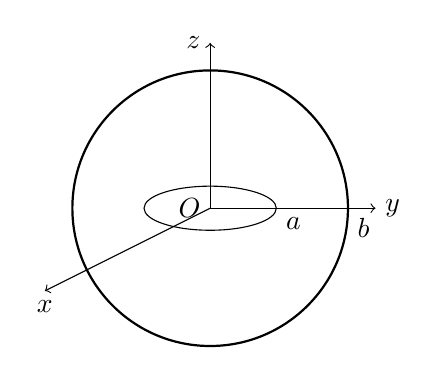
\begin{tikzpicture}[scale=.7]
            \draw[<->](0, 3)node[left]{$z$}--(0, 0)node[left]{$O$}--(3, 0)node[right]{$y$};
            \draw[->](0, 0)--(-3, -1.5)node[below]{$x$};
            \draw[thick](0, 0)circle(2.5);
            \node[below right]at(2.5, 0){$b$};
            \draw(0, 0)ellipse(1.2 and .4);
            \node[below right]at(1.2, 0){$a$};
        \end{tikzpicture}
        \tikzchap 接地球内带电圆环
    \end{center}
    \fi
    环的电荷密度可以写成
    \[
        \rho(\bm x')=\frac Q{2\pi a^2}\vd(r'-a)\vd(\cos\theta').
    \]
    由方位角的对称性,$m=0$,故
    \begin{align*}
        \Phi(\bm x)&=\frac1{4\pi\varepsilon_0}\int\rho(\bm x')G(\bm x,\bm x')\d v'\\
        &=\frac Q{4\pi\varepsilon_0}\sum_{\ell=0}^\infty\biggkh{\frac{r_<^\ell}{r_>^{\ell+1}}-\frac{r^\ell a^\ell}{b^{2\ell+1}}}P_\ell(\cos\theta)P_\ell(0)\\
        &=\frac Q{4\pi\varepsilon_0}\sum_{n=0}^\infty\frac{(-)^n(2n-1)!!}{(2n)!!}\biggkh{\frac{r_<^{2n}}{r_>^{2n+1}}-\frac{r^{2n}a^{2n}}{b^{4n+1}}}P_{2n}(\cos\theta).
    \end{align*}
\end{example}

\subsection{柱坐标系下Green函数的展开}
\label{ssec: Green expansion in cylindrical coordinate}

柱坐标系下,
\[
    \lapla G(\bm x,\bm x')=-\frac{4\pi}\rho\vd(\rho-\rho')\vd(\phi-\phi')\vd(z-z').
\]
Green函数可以写成
\[
    G(\bm x,\bm x')=\frac1{4\pi^2}\sum_{m=-\infty}^\infty\int\iti\e{\i m(\phi-\phi')}\e{\i k(z-z')}g_m(k,\rho,\rho')\d k.
\]
径向Green函数$g_m(k,\rho,\rho')$
\begin{equation}
    \label{eqn:cylinder green}
    \frac1\rho\dd\rho\biggkh{\rho\dv{g_m}\rho}-\biggkh{k^2+\frac{m^2}{\rho^2}}g_m=-\frac{4\pi}\rho\vd(\rho-\rho').
\end{equation}
当$\rho\neq\rho'$时,上式为修正Bessel方程,解为$I_m(k\rho),\,K_m(k\rho)$,由对称性
\[
    g_m(k,\rho,\rho')=\psi_1(k\rho_<)\psi_2(k\rho_>).
\]
$\psi_1,\psi_2$是$I_m,K_m$的线性组合。由方程右边$\delta$函数所隐含的斜率不连续条件:
\[
    \edg{\dv{g_m}\rho}_{\rho'+\epsilon}-\edg{\dv{g_m}\rho}_{\rho'-\epsilon}=kW[\psi_1,\psi_2]=-\frac{4\pi}\rho.
\]
其中Wro\'nski行列式(Wronskian) $W[\psi_1,\psi_2]=\psi_1\psi_2'-\psi_2\psi_1'$,由于方程\eqref{eqn:cylinder green}是Strum-Liouville型的:
\[
    \dd x\biggfkh{p(x)\dv yx}+g(x)y=0,
\]
故其两线性独立解的Wronskian $\propto 1/p(x)$,因此我们可以找到一个满足所有$\rho'$的解,我们必须要求归一化$\psi_1\psi_2$使得Wronskian
\[
    W[\psi_1(x),\psi_2(x)]=-\frac{4\pi}x.
\]
如果没有边界,$g_m(k,\rho,\rho')$必须在$\rho=0$处收敛且在$\rho\to\infty$趋于0,由此$\psi_1(k\rho)=AI_m(k\rho),\,\psi_2(k\rho)=K_m(k\rho)$,又
\[
    W[I_m(x),K_m(x)]=-\frac1x,
\]
故$A=4\pi$,我们得到了$1/|\bm x-\bm x'|$的展开 
\begin{equation}
    \frac1{|\bm x-\bm x'|}=\frac1\pi\sum_{m=-\infty}^{+\infty}\int\iti\e{\i m(\phi-\phi')}\e{\i k(z-z')}I_m(k\rho_<)K_m(k\rho_>)\d k.
\end{equation}

\subsection{Green函数的本征函数展开式}
\label{ssec:eigenfunction expansions for Green functions}

另一种获得Green函数展开式的技术是在一些相关问题上使用本征函数(eigenfunction)。作为说明,我们考虑一个椭圆微分方程的形式
\begin{equation}
    \lapla\psi(\bm x)+\bigfkh{f(\bm x)+\lambda}\psi(\bm x)=0.
\end{equation}
为了使本征函数$\psi_n(\bm x)$满足边界条件,$\lambda$必须取一系列本征值$\lambda_n$。
%\lapla\psi_n(x)+\bigfkh{f(x)+\lambda_n}\psi_n(x)=0.

本征函数是正交的:
\[
    \int_V\psi_m^\ast(\bm x)\psi_n(\bm x)\d v=\vd_{mn}.
\]
本征值$\lambda$的谱可以是离散集,也可以是连续集,或者两者兼而有之。我们假定所有本征函数构成一个完备集。

现在我们希望找到Green函数的方程:
\begin{equation}
    \lapla G(\bm x,\bm x')+\bigfkh{f(\bm x)+\lambda}G(\bm x,\bm x')=-4\pi\vd(\bm x,\bm x'),
\end{equation}
若Green函数与的本征函数$\psi_n(\bm x)$具有相同的边界条件,则可将Green函数展开为一系列本征函数的形式:
\[
    G(\bm x,\bm x')=\sum_n a_n(\bm x')\psi_n(\bm x),
\]
代入得
\[
    \sum_n a_n(\bm x')(\lambda-\lambda_n)\psi_n=-4\pi\vd(\bm x,\bm x'),
\]
因此系数为
\[
    a_n(\bm x')=\frac{4\pi}{\lambda_n-\lambda}\int_V\psi^\ast_n(\bm x)\vd(\bm x,\bm x')\d v=4\pi\frac{\psi_n^\ast(\bm x')}{\lambda_n-\lambda}.
\]
因此Green函数的本征函数展开式为
\begin{equation}
    G(\bm x,\bm x')=4\pi\sum_n \frac{\psi_n^\ast(\bm x')\psi_n(\bm x)}{\lambda_n-\lambda}
\end{equation}
对于连续谱,求和用积分代替。
\begin{example}{$1/|\bm x-\bm x'|$的三维Fourier积分表示}{1/|x-x'| Fourier}
    自由边界下,$f(\bm x)\equiv 0$的特征方程
    \[
        (\lapla+k^2)\psi_{\bm k}(\bm x)=0\implies\psi_{\bm k}(\bm x)=\frac{\e{\i\bm k\cdot\bm x}}{(2\pi)^{3/2}}.
    \]
    则$\lambda=0$时的Green函数为
    \[
        G(\bm x,\bm x')=4\pi\int\frac{\psi_{\bm k}^\ast(\bm x')\psi_{\bm k}(\bm x)}{k^2}\d v_k=\frac1{2\pi^2}\int\frac{\e{\i\bm k\cdot(\bm x'-\bm x)}}{k^2}\d v_k.
    \]
\end{example}

\sectionstar{混合边界条件}
\label{sec:mixed boundary condition}

Jackson举例了带一圆孔的导电平板问题,略。

